\subsection{\RU{Забудем на время о MSVC}\EN{Let's forget about MSVC}}

\RU{\ac{SEH} в Windows предназначен для обработки исключений, тем не менее, с \Cpp и \ac{OOP} он никак не связан}
\EN{In Windows, \ac{SEH} is intended for exceptions handling, nevertheless, it is language-agnostic,
it is not related to the \Cpp or \ac{OOP} in any way}.
\RU{Здесь мы рассмотрим \ac{SEH} изолированно от Си++ и расширений MSVC}
\EN{Here we will take a look on \ac{SEH} in isolated (from C++ and MSVC extensions) form}.

\index{Windows!TIB}
\index{Windows!Win32!RaiseException()}
\RU{Каждый процесс имеет цепочку \ac{SEH}-обработчиков, и адрес последнего записан в \ac{TIB}}
\EN{Each running process has a chain of \ac{SEH}-handlers, \ac{TIB} has address of the last handler}.
\RU{Когда происходит исключение (деление на ноль, обращение по неверному адресу в памяти, 
пользовательское исключение, поднятое при помощи \TT{RaiseException()}),
\ac{OS} находит последний обработчик в \ac{TIB} и вызывает его, 
передав ему информацию о состоянии \ac{CPU} в момент исключения
(все значения регистров, и т.д.)}
\EN{When exception occurred (division by zero, incorrect address access, user exception triggered by
calling to \TT{RaiseException()} function), \ac{OS} will find the last handler in \ac{TIB}, and will call it
with passing all information about \ac{CPU} state (register values, etc) at the moment of exception}.
\RU{Обработчик выясняет, то ли это исключение, для которого он создавался}\EN{Exception handler will
consider exception, was it made for it}?
\RU{Если да, то он обрабатывает исключение}\EN{If so, it will handle exception}.
\RU{Если нет, то показывает \ac{OS} что он не может его обработать и \ac{OS} вызывает следующий обработчик
в цепочке, и так до тех пор, пока не найдется обработчик способный обработать исключение}
\EN{If no, it will signal to \ac{OS} that it
cannot handle it and \ac{OS} will call next handler in chain,
until a handler which is able to handle the exception will be found}.

\RU{В самом конце цепочки находится стандартный обработчик, показывающий всем очень известное окно, 
сообщающее что процесс упал, 
сообщает также состояние \ac{CPU} в момент падения и позволяет собрать и отправить информацию обработчикам 
в Microsoft}
\EN{At the very end of the chain, there a standard handler, showing well-known dialog box, informing a
process crash, some technical information about \ac{CPU} state at the crash,
and offering to collect all information and send it to developers in Microsoft}. 

\begin{figure}[H]
\centering
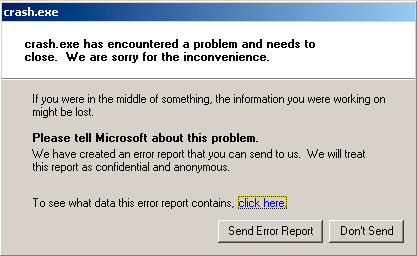
\includegraphics[scale=0.66]{OS/SEH/1/crash_xp1.png}
\caption{Windows XP}
\end{figure}

\begin{figure}[H]
\centering
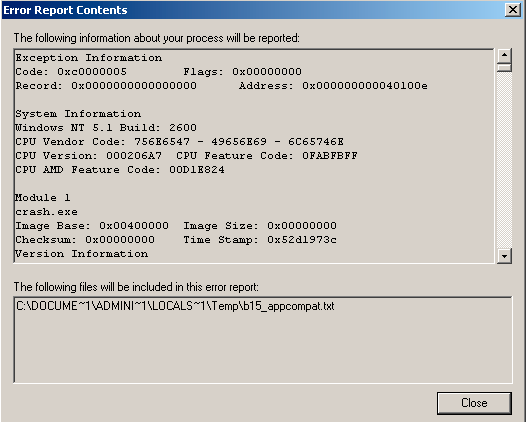
\includegraphics[scale=0.66]{OS/SEH/1/crash_xp2.png}
\caption{Windows XP}
\end{figure}

\begin{figure}[H]
\centering
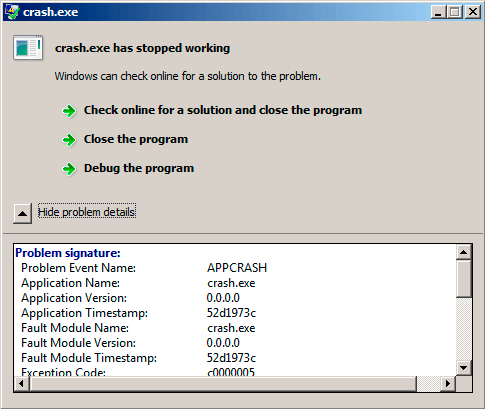
\includegraphics[scale=0.66]{OS/SEH/1/crash_win7.png}
\caption{Windows 7}
\end{figure}

\begin{figure}[H]
\centering
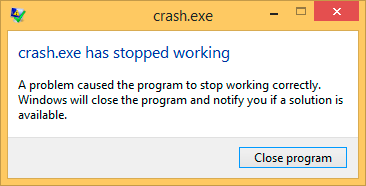
\includegraphics[scale=0.66]{OS/SEH/1/crash_win81.png}
\caption{Windows 8.1}
\end{figure}

\RU{Раньше этот обработчик назывался Dr. Watson}\EN{This handler was also called Dr. Watson earlier}
\footnote{\url{http://go.yurichev.com/17046}}.

\RU{Кстати, некоторые разработчики делают свой собственный обработчик,
отправляющий информацию о падении программы им самим}
\EN{By the way, some developers made their own handler, sending information about program crash to themselves}.
\index{Windows!Win32!SetUnhandledExceptionFilter()}
\RU{Он регистрируется при помощи ф-ции}\EN{It is registered with the help of} \TT{SetUnhandledExceptionFilter()} 
\RU{и будет вызван если \ac{OS} не знает как иначе обработать исключение}\EN{and will be called if
\ac{OS} do not have any other way to handle exception}.
\index{\oracle}
\RU{А, например,}\EN{Other example is} \oracle \RU{в этом случае генерирует огромные дампы, 
содержащие всю возможную информацию и состоянии \ac{CPU} и памяти}
\EN{it saves huge dumps containing all possible information about \ac{CPU} and memory state}.

\RU{Попробуем написать свой примитивный обработчик исключений}
\EN{Let's write our own primitive exception handler}
\footnote{
	\RU{Пример основан на примере из}\EN{The example is based on the example from} \cite{PietrekSEH}

	\RU{Он должен компилироваться с опцией}\EN{It is compiled with the} SAFESEH\EN{ option}: 
	\TT{cl seh1.cpp /link /safeseh:no}

	\RU{Подробнее об опции}\EN{More about} SAFESEH \RU{здесь}\EN{here}: \\
	\url{http://msdn.microsoft.com/en-us/library/9a89h429.aspx}
}:
	
\lstinputlisting{OS/SEH/1/1.cpp}

\RU{Сегментный регистр FS: в win32 указывает на \ac{TIB}}
\EN{FS: segment register is pointing to the \ac{TIB} in win32}.
\RU{Самый первый элемент \ac{TIB} это указатель на последний обработчик в цепочке}
\EN{The very first element in \ac{TIB} is a pointer to the last handler in chain}.
\RU{Мы сохраняем его в стеке и записываем туда адрес своего обработчика}\EN{We saving it in the stack and store
an address of our handler there}.
\RU{Эта структура называется}\EN{The structure is named} \TT{\_EXCEPTION\_REGISTRATION}, 
\RU{это простейший односвязный список, и эти элементы хранятся прямо в стеке}\EN{it is a simplest singly-linked
list and its elements are stored right in the stack}.

\begin{lstlisting}[caption=MSVC/VC/crt/src/exsup.inc]
\_EXCEPTION\_REGISTRATION struc
     prev    dd      ?
     handler dd      ?
\_EXCEPTION\_REGISTRATION ends
\end{lstlisting}

\RU{Так что каждое поле}\EN{So each} ``handler'' \RU{указывает на обработчик,
а каждое поле}\EN{field points to handler and an each} ``prev'' \RU{указывает на предыдущую структуру
в стеке}\EN{field points to previous record in the stack}.
\RU{Самая последняя структура имеет}\EN{The last record has} \TT{0xFFFFFFFF} (-1) \RU{в поле}\EN{in} 
``prev''\EN{ field}.

\begin{center}
\ifdefined\ebook
\begin{tikzpicture}[thick,scale=0.50, every node/.style={scale=0.50}]
\else
\begin{tikzpicture}[thick,scale=0.85, every node/.style={scale=0.85}]
\fi
	\tikzstyle{every path}=[thick]
	\tikzstyle{undefined}=[draw,rectangle,minimum height=1cm, minimum width=3.5cm, text width=3.5cm]
	\tikzstyle{node}=[draw,rectangle,minimum height=1cm, minimum width=3.5cm, text width=3.5cm, fill=gray!20]
	
	\node[node] (fs) [minimum width=1.5cm, text width=1.5cm] {FS:0};

	\node[node] (tib1) [right=1.5cm of fs] {+0: \_\_except\_list};
	\node[undefined] (tib2) [below of=tib1] {+4: \dots};
	\node[undefined] (tib3) [below of=tib2] {+8: \dots};
	\node (tib_text) [above of=tib1] {TIB};
	
	\draw [->] (fs.east) -- (tib1.west);

	\node[undefined] (u1) [text centered, right=2.5cm of tib1] {\dots};
	\node [node] (n1prev) [below of=u1] {Prev=0xFFFFFFFF};
	\node [node] (n1handler) [below of=n1prev] {Handle};
	\node [node] (n1handler_text) [right=1cm of n1handler] {\HandlerFunction};
	\draw [->] (n1handler.east) -- (n1handler_text.west);
	\node[undefined] (u2) [text centered, below of=n1handler] {\dots};
	\node [node] (n2prev) [below of=u2] {Prev};
	\node [node] (n2handler) [below of=n2prev] {Handle};
	\node [node] (n2handler_text) [right=1cm of n2handler] {\HandlerFunction};
	\draw [->] (n2handler.east) -- (n2handler_text.west);
	\node[undefined] (u3) [text centered, below of=n2handler] {\dots};
	\node [node] (n3prev) [below of=u3] {Prev};

	\node [node] (n3handler) [below of=n3prev] {Handle};
	\node [node] (n3handler_text) [right=1cm of n3handler] {\HandlerFunction};
	\draw [->] (n3handler.east) -- (n3handler_text.west);
	\node[undefined] (u4) [text centered, below of=n3handler] {\dots};
	\node (stack_text) [above of=u1] {\IFRU{Стек}{Stack}};
	
	\node (n2block_pt1) [inner sep=0pt, above left=0cm and 0cm of n2prev] {};
	\node (n2block_pt2) [inner sep=0pt, above left=0cm and 0.5cm of n2prev] {};
	\draw [->] (n3prev.west) .. controls +(left:0.5cm) and (n2block_pt2) .. (n2block_pt1);

	\node (n1block_pt1) [inner sep=0pt, above left=0cm and 0cm of n1prev] {};
	\node (n1block_pt2) [inner sep=0pt, above left=0cm and 0.8cm of n1prev] {};
	\draw [->] (n2prev.west) .. controls +(left:0.8cm) and (n1block_pt2) .. (n1block_pt1);
	
	\node (n3block_pt1) [inner sep=0pt, above left=0cm and 0cm of n3prev] {};
	\node (n3block_pt2) [inner sep=0pt, above left=0cm and 1.25cm of n3prev] {};
	\draw [->] (tib1.east) .. controls +(right:1.25cm) and (n3block_pt2) .. (n3block_pt1);


\end{tikzpicture}
\end{center}


\RU{После инсталляции своего обработчика, вызываем}\EN{When our handler is installed, let's call}
\TT{RaiseException()}
\footnote{\url{http://msdn.microsoft.com/en-us/library/windows/desktop/ms680552(v=vs.85).aspx}}.
\RU{Это пользовательские исключения}\EN{This is user exception}. \RU{Обработчик проверяет код}\EN{Handler will check
the code}.
\RU{Если код}\EN{If the code is} \TT{0xE1223344}, \RU{то он возвращает}\EN{it will return} 
\TT{ExceptionContinueExecution},
\RU{что сигнализирует системе что обработчик скорректировал состояние CPU (обычно это регистры EIP/ESP) и что OS может
возобновить исполнение треда}
\EN{which means that handler corrected CPU state (it is usually correction of EIP/ESP registers) and the OS can resume thread execution}.
\RU{Если вы немного измените код так что обработчик будет возвращать}\EN{If to alter the code slightly
so the handler will return} \TT{ExceptionContinueSearch},
\RU{то \ac{OS} будет вызывать остальные
обработчики в цепочке, и врядли найдется тот, кто обработает ваше исключение,
ведь информации о нем (вернее, его коде) ни у кого нет}
\EN{then \ac{OS} will call other handlers, and very unlikely the one who can handle it will be founded, since
no one have information about it (rather about its code)}.
\RU{Вы увидите стандартное окно Windows о падении процесса}\EN{You will see the standard Windows dialog about
process crash}.

\RU{Какова разница между системными исключениями и пользовательскими}\EN{What is the difference between
system exceptions and user}? \RU{Вот системные}\EN{Here is a system ones}:

\begin{center}
\begin{tabular}{ | l | l | l | }
\hline
\cellcolor{blue!25} \RU{как определен в}\EN{as defined in} WinBase.h & 
\cellcolor{blue!25} \RU{как определен в}\EN{as defined in} ntstatus.h & 
\cellcolor{blue!25} \RU{численное значение}\EN{numerical value} \\
\hline
EXCEPTION\_ACCESS\_VIOLATION          & STATUS\_ACCESS\_VIOLATION           & 0xC0000005 \\
\hline
EXCEPTION\_DATATYPE\_MISALIGNMENT     & STATUS\_DATATYPE\_MISALIGNMENT      & 0x80000002 \\
\hline
EXCEPTION\_BREAKPOINT                & STATUS\_BREAKPOINT                 & 0x80000003 \\
\hline
EXCEPTION\_SINGLE\_STEP               & STATUS\_SINGLE\_STEP                & 0x80000004 \\
\hline
EXCEPTION\_ARRAY\_BOUNDS\_EXCEEDED     & STATUS\_ARRAY\_BOUNDS\_EXCEEDED      & 0xC000008C \\
\hline
EXCEPTION\_FLT\_DENORMAL\_OPERAND      & STATUS\_FLOAT\_DENORMAL\_OPERAND     & 0xC000008D \\
\hline
EXCEPTION\_FLT\_DIVIDE\_BY\_ZERO        & STATUS\_FLOAT\_DIVIDE\_BY\_ZERO       & 0xC000008E \\
\hline
EXCEPTION\_FLT\_INEXACT\_RESULT        & STATUS\_FLOAT\_INEXACT\_RESULT       & 0xC000008F \\
\hline
EXCEPTION\_FLT\_INVALID\_OPERATION     & STATUS\_FLOAT\_INVALID\_OPERATION    & 0xC0000090 \\
\hline
EXCEPTION\_FLT\_OVERFLOW              & STATUS\_FLOAT\_OVERFLOW             & 0xC0000091 \\
\hline
EXCEPTION\_FLT\_STACK\_CHECK           & STATUS\_FLOAT\_STACK\_CHECK          & 0xC0000092 \\
\hline
EXCEPTION\_FLT\_UNDERFLOW             & STATUS\_FLOAT\_UNDERFLOW            & 0xC0000093 \\
\hline
EXCEPTION\_INT\_DIVIDE\_BY\_ZERO        & STATUS\_INTEGER\_DIVIDE\_BY\_ZERO     & 0xC0000094 \\
\hline
EXCEPTION\_INT\_OVERFLOW              & STATUS\_INTEGER\_OVERFLOW           & 0xC0000095 \\
\hline
EXCEPTION\_PRIV\_INSTRUCTION          & STATUS\_PRIVILEGED\_INSTRUCTION     & 0xC0000096 \\
\hline
EXCEPTION\_IN\_PAGE\_ERROR             & STATUS\_IN\_PAGE\_ERROR              & 0xC0000006 \\
\hline
EXCEPTION\_ILLEGAL\_INSTRUCTION       & STATUS\_ILLEGAL\_INSTRUCTION        & 0xC000001D \\
\hline
EXCEPTION\_NONCONTINUABLE\_EXCEPTION  & STATUS\_NONCONTINUABLE\_EXCEPTION   & 0xC0000025 \\
\hline
EXCEPTION\_STACK\_OVERFLOW            & STATUS\_STACK\_OVERFLOW             & 0xC00000FD \\
\hline
EXCEPTION\_INVALID\_DISPOSITION       & STATUS\_INVALID\_DISPOSITION        & 0xC0000026 \\
\hline
EXCEPTION\_GUARD\_PAGE                & STATUS\_GUARD\_PAGE\_VIOLATION       & 0x80000001 \\
\hline
EXCEPTION\_INVALID\_HANDLE            & STATUS\_INVALID\_HANDLE             & 0xC0000008 \\
\hline
EXCEPTION\_POSSIBLE\_DEADLOCK         & STATUS\_POSSIBLE\_DEADLOCK          & 0xC0000194 \\
\hline
CONTROL\_C\_EXIT                      & STATUS\_CONTROL\_C\_EXIT             & 0xC000013A \\
\hline
\end{tabular}
\end{center}

\RU{Так определяется код}\EN{That is how the code is defined}:

\begin{center}
\begin{bytefield}[bitwidth=0.03\linewidth]{32}
\bitheader[endianness=big]{31,29,28,27,16,15,0} \\
\bitbox{2}{\TT{S}} & 
\bitbox{1}{\TT{U}} &
\bitbox{1}{0} & 
\bitbox{12}{Facility code} &
\bitbox{16}{Error code}
\end{bytefield}
\end{center}

S \RU{это код статуса}\EN{is a basic status code}: 
11\EMDASH{}\RU{ошибка}\EN{error};
10\EMDASH{}\RU{предупреждение}\EN{warning};
01\EMDASH{}\RU{информация}\EN{informational};
00\EMDASH{}\RU{успех}\EN{success}.
U\EMDASH\RU{является ли этот код пользовательским, а не системным}\EN{whether the code is user code}.

\RU{Вот почему я выбрал}\EN{That is why I chose} 0xE1223344\EMDASH{}
%E\textsubscript{16} (1110\textsubscript{2}) 
0xE (1110b) 
\RU{означает что это 1) пользовательское исключение; 2) ошибка}\EN{mean this is 1) user exception; 2) error}.
\RU{Хотя, если быть честным, этот пример нормально работает и без этих старших бит}
\EN{But to be honest, this example works finely without these high bits}.

\RU{Далее мы пытаемся прочитать значение из памяти по адресу 0}\EN{Then we try to read a value from memory
at the 0th address}.
\RU{Конечно, в win32 по этому адресу обычно ничего нет, и сработает исключение}
\EN{Of course, there are nothing at this address in win32, so exception is raised}.
\RU{Однако, первый обработчик, который будет заниматься этим делом ~--- ваш, и он узнает об этом
первым, проверяя код на соответствие с константной \TT{EXCEPTION\_ACCESS\_VIOLATION}}
\EN{However, the very first handler will be called --- yours, it will be notified first, checking
the code on equality to the \TT{EXCEPTION\_ACCESS\_VIOLATION} constant}.

\RU{А если заглянуть в то что получилось на ассемблере,
то можно увидеть что код читающий из памяти по адресу 0, выглядит так}\EN{The code reading from memory at
0th address is looks like}:

\lstinputlisting[caption=MSVC 2010]{OS/SEH/1/1_fragment.asm}

\RU{Возможно ли ``на лету'' исправить ошибку и предложить программе исполняться далее}
\EN{Will it be possible to fix error ``on fly'' and to continue program execution}?
\RU{Да, наш обработчик может изменить значение в \EAX и предложить \ac{OS} исполнить эту же инструкцию еще раз}
\EN{Yes, our exception handler can fix \EAX value and now let \ac{OS} will execute this instruction once again}.
\RU{Что мы и делаем}\EN{So that is what we do}. \printf \RU{напечатает}\EN{will print} 1234,
\RU{потому что после работы нашего обработчика}\EN{because, after execution of our handler},
\EAX \RU{будет не}\EN{will not be} 0,
\RU{а будет содержать адрес глобальной переменной}\EN{it will contain address of global variable} \TT{new\_value}.
\RU{Программа будет исполняться далее}\EN{Execution will be resumed}.

\RU{Собственно, вот что происходит}\EN{That is what is going on}: 
\RU{срабатывает защита менеджера памяти в \ac{CPU}}\EN{memory manager in \ac{CPU} signaling about error}, 
\RU{он останавливает работу треда}\EN{the \ac{CPU} suspends the thread},
\RU{отыскивает в ядре Windows обработчик исключений}\EN{it finds exception handler in the Windows kernel}, 
\RU{тот, в свою очередь, начинает вызывать обработчики из цепочки \ac{SEH}, по одному}
\EN{latter, in turn, is starting to call all handlers in \ac{SEH} chain, one by one}.

\RU{Я компилирую это всё в MSVC 2010, но конечно же, нет никакой гарантии 
что для указателя будет использован именно регистр \EAX}\EN{I use MSVC 2010 now, but of course,
there are no any guarantee that \EAX will be used for pointer}.

\RU{Этот трюк с подменой адреса эффектно выглядит, 
и я его привожу здесь для наглядной иллюстрации работы \ac{SEH}}
\EN{This address replacement trick is looks showingly, and I offer it here for \ac{SEH} internals illustration}.
\RU{Тем не менее, я затрудняюсь
припомнить, применяется ли где-то подобное на практике для исправления ошибок ``на лету''}
\EN{Nevertheless, I cannot recall
where it is used for ``on-fly'' error fixing in practice}.

\RU{Почему SEH-записи хранятся именно в стеке а не в каком-то другом месте}
\EN{Why SEH-related records are stored right in the stack instead of some other place}?
\RU{Вероятно, потому что тогда \ac{OS} не будет заботиться об освобождении этой информации, эти записи
пропадают как ненужные когда ф-ция заканчивает работу}
\EN{Supposedly because then \ac{OS} will not need to care about freeing this information, these records
will be disposed when function finishing its execution}.
\RU{Но я не уверен на}\EN{But I'm not} 100\%\RU{ и могу ошибаться}\EN{-sure and can be wrong}.
\index{\CStandardLibrary!alloca()}
\RU{Это чем-то похоже на}\EN{This is somewhat like} alloca(): (\ref{alloca}).

